% Created 2018-01-27 Sat 18:02
\documentclass{article}
\usepackage[utf8]{inputenc}
\usepackage[T1]{fontenc}
\usepackage{fixltx2e}
\usepackage{graphicx}
\usepackage{longtable}
\usepackage{float}
\usepackage{wrapfig}
\usepackage{rotating}
\usepackage[normalem]{ulem}
\usepackage{amsmath}
\usepackage{textcomp}
\usepackage{marvosym}
\usepackage{wasysym}
\usepackage{amssymb}
\usepackage{hyperref}
\tolerance=1000
\usepackage[margin=1in]{geometry}
\author{Shannon Gallagher}
\date{\today}
\title{Catalyst: Agents of Change}
\hypersetup{
  pdfkeywords={},
  pdfsubject={},
  pdfcreator={Emacs 25.3.1 (Org mode 8.2.10)}}
\begin{document}

\maketitle


\section{Outline of software}
\label{sec-1}
\begin{verbatim}
INPUT: Control file with agents file; disease parameters;
 disease model; time steps; parallel options;
 activity schedule; individual agents/instantiations to track
for every time step t
  for every activity at time t
    prob_infection = infect_agents(agents, activity, 
                     time, disease)
  end
  agent_status = update_agents(prob_infection)
  update_activities()
  update_disease()
end
OUTPUT: status of agent at each time step, saved as multiple text files;
 number of agents in compartment at each time step;
 specific agents over time; activity info
\end{verbatim}

\subsection{Infect Agents}
\label{sec-1-1}
\begin{verbatim}
INPUT: agents, activity, time, disease
for every infected agent ii
  for every neighbor of agent ii, jj
    update_infection_prob(ii,jj, activity, disease, time)
  end
end
OUTPUT: updated agent probabilities
\end{verbatim}

\section{Description}
\label{sec-2}
\subsection{General Outline}
\label{sec-2-1}


The benefit of this program is that the agent-based part (the infect\_agents portion) is completely modular.  The function update\_agents() is a multinomial draw.  Thus this portion can be used both for heterogeneous individual agents along with homogeneous agents (the compartment-model).

\subsection{Infect Agents -- the "AM" portion}
\label{sec-2-2}
This function is what differentiates the model from a CM. In this step, agents explicitly interact with one another and hence can change one another.  This interaction has the potential to be very slow.  Naively, if we were to loop over all pairs of agents and all environments then we would be looking at $O(N^2E)$ run-time where $N$ is the number of agents and $E$ is the number of environments.

Hence, it is critical to be speed up this step.  It is worth noting that in the SI-framework, the only interactions that are worthwhile is when an agent is actively infecting another.  All other compartment transitions are independent from one another, meaning they do not depend on the status of other agents.  Hence we only need to loop over agents in "infectious" states.  Moreover, we only need to look at the neighbors' of these infectious agents, specifically those in susceptible states.

We also assume that once an agent is infected by another, she will be unaffected by further infections.  As such, once an agent is infected by another, we remove her from the susceptible pool.

We plan to reduce this step to $O(I)$ where $I$ is the number of infectious individuals where, typically $I << N$.  The first step is that we only need to loop over infectious agents, for a run time of $O(I)$.  We then need to loop over all neighbors of infectious agents.  However, we note that we can pre-compute potential neighbors and store them in a dictionary, so look up will be $O(1)$.  Neighbors will be over all environments so we no longer have to loop over those.  Thus we only have to check whether neighbors of the infectious are susceptible and update the infection probabilities based on the environment activities, pair of interacting agents, and disease parameters.


\subsection{Working Prototype v0.0.1}
\label{sec-2-3}
I have implemented the code in the general outline as \texttt{catalyst v0.0.1}.

Specifically, I am using 10 agents with 3 environments.  Agents with an environment assignment of 0 are considered null assignments (e.g. the agent does not attend school).  The 3 compartments are Susceptible, Infectious, and Recovered.  In this model, there is a 100\% chance of an infectious agent infecting their neighbors.  Once infectious, an agent has a 50\% chance of recovery at each time step.  All recovered agents remain in that state.

The results are displayed in Figure \ref{fig:working-prototype}, where the first 9 agents are initially susceptible (blue) and the 10th agent is infectious (red).  We can glimpse some sense of the neighbor structure in the next step ($t=1$) as we see agents 6-9 are all infected by agent 10.  Agent 10 recovers at time $t=1$.  Then agents 6-9 infect agents 2-5 at time $t=2$.  All agents 2-10 end up recovering by time $t=6$.  We see agent 1 escapes infection completely because it has no neighbors.

The \textbf{output} of my program is a csv with dimension $T \times N$ where entry $t,n$ is the agent $n$'s status at time $t$.

\subsubsection{Modular parts}
\label{sec-2-3-1}
Although the above working prototype is simple, it is modular in many aspects.

\begin{enumerate}
\item \textbf{Compartments}.  The user can identify arbitrarily many compartments.  The only requirement is that some compartments must be of class "susceptible" and at least one compartment is an "infectious" agent.

\item \textbf{Base probabilities}.  This is a 3D array of size $K\times K \times T$ where $K$ is the number of compartments and $T$ is the total number of time steps.  Here entry $i,j,t$ is the probability of an agent in state $i$ transitioning to state $j$ at time $t$ to $t+1$.  These base probabilities, may be set, for instance, to the CM probabilities specified in my proposal.  These serve as default transitions.  And since $K << N$ in general, the memory and/or the computational time required to compute these probabilities is relatively small.

\item \textbf{Conditional agent probabilities}.  Instead of storing probabilities of transition at each time step and for every possible state the agent is in, we only store a single time step at a time, conditioned on the agent's current compartment.  This is a $N \times K$ array where $N$ is the total number of agents and $K$ is the total number of compartments.  Then entry $n,k$ is agent $n$'s probability of transitioning to compartment $k$ given it's current compartment.  These conditional agent probabilities are by default, taken from the base probabilities.  However, these can be updated through the "AM portion" of \texttt{catalyst} to allow for individual interactions to take effect.

\item \textbf{Environmental and disease properties}.  Environment and disease properties are included (although currently without effect) so in the future environment closings and dynamic disease properties may be added into the program.
\end{enumerate}



\begin{figure}[H]
\center
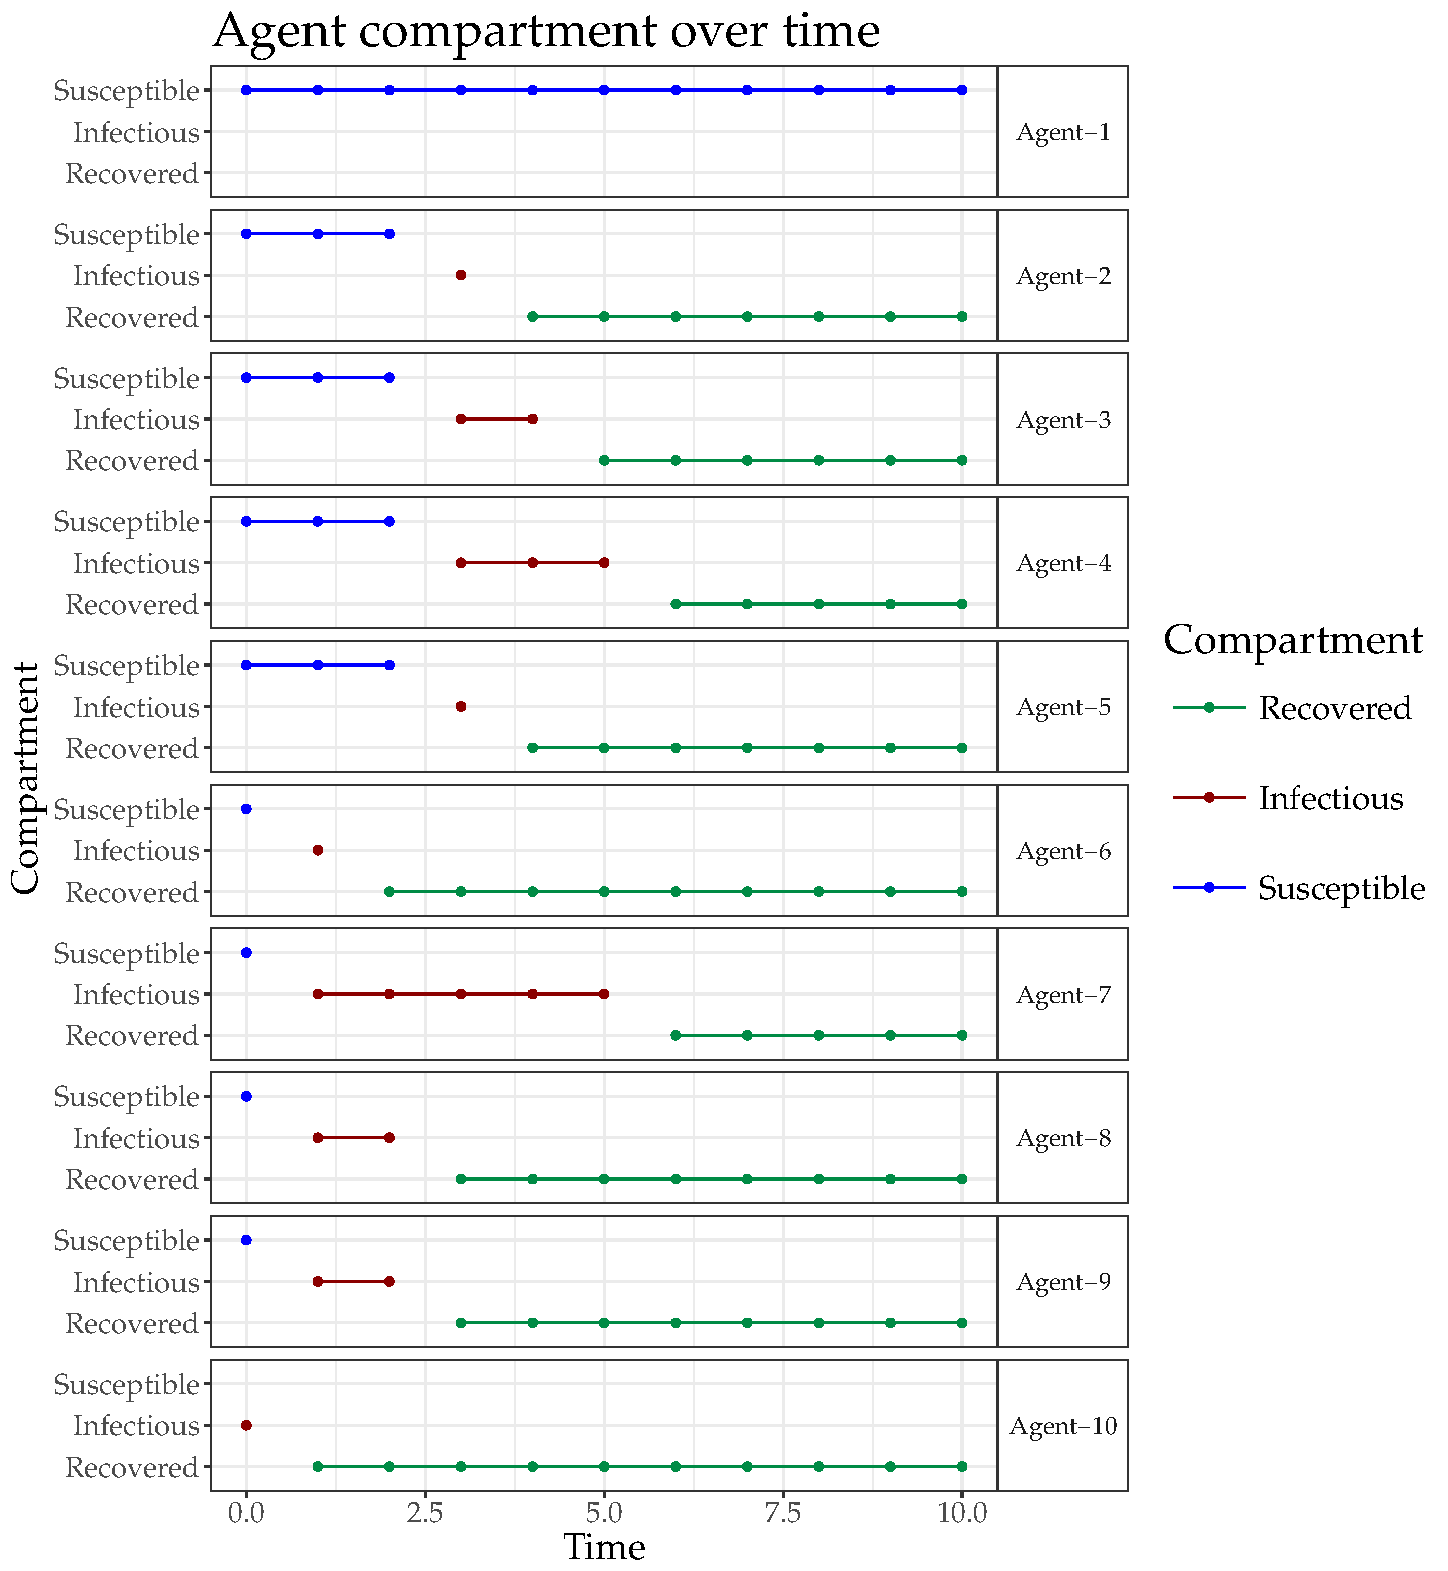
\includegraphics[width=\textwidth]{images/agents-plot.pdf}
\caption{Prototype of catalyst with one infectious agent at time t=0.}\label{fig:working-prototype}
\end{figure}

\section{Current implementation}
\label{sec-3}
\begin{itemize}
\item A working framework in C
\item Incorporation of GNU Standard Library packages for ODE integration and random number generation
\item A working SIR model
\item Testing framework to initialize agents and environments
\item A Dictionary of neighbors through GLib's GHashTable
\item Working prototype
\end{itemize}

\section{Next Steps}
\label{sec-4}
\begin{itemize}
\item Integrate ODE probabilities into model as base probabilities
\item Fit ODE models
\begin{itemize}
\item Fit a SIR ODE model after the the AM part is run
\item Fit a SEIR ODE model
\item Attempt to make framework to fit generic model
\end{itemize}
\item Run for a number of repetitions
\begin{itemize}
\item Should be able to share pre-computations like base probabilities and neighbor dictionary
\end{itemize}
\item Option to summarize output instead of saving everything
\item Way to track who infects whom (to estimate R0 down the line)
\end{itemize}




\section{Long Term}
\label{sec-5}
\begin{itemize}
\item Input file standards
\item Make the ODE solver more generic to support general systems.  The main problem is how to incorporate this symbolically to be an easy input for the control file
\item Estimate ODE parameters from an AM through least squares or mle.
\item Convert SPEW agents to a viable format for catalyst
\item Make nice interface for control file (shiny)
\item Parallelization
\item Visualize outputs
\end{itemize}

\section{Schedule}
\label{sec-6}
\subsection{{\bfseries\sffamily DONE} \textit{<2018-01-01 Mon>} - \textit{<2018-01-13 Sat>}}
\label{sec-6-1}
\begin{itemize}
\item Set up preliminaries.
\item Learned how to use C libraries, especially GSL (GNU Scientific Library).
\item Got a much clearer demonstration of how pointers work
\item "Finalize" framework for software
\end{itemize}

\subsection{{\bfseries\sffamily DONE} \textit{<2018-01-15 Mon>} - \textit{<2018-01-21 Sun>}}
\label{sec-6-2}
\subsubsection{The "AM" part}
\label{sec-6-2-1}
\begin{itemize}
\item set up testing framework for cm-am
\item Work and get used to GLib and included data structures including Arrays which can grow, singly-linked lists, and hashtables to use within C.
\item Made a function to make a dictionary of neighbors.
\end{itemize}
\subsection{{\bfseries\sffamily DONE} \textit{<2018-01-22 Mon>} - \textit{<2018-01-26 Fri>}}
\label{sec-6-3}
\begin{itemize}
\item Store both a single probability and multiple probabilities for agents, \ldots{} likely not stored at each step
\item Visualize outputs in R
\end{itemize}
\subsection{{\bfseries\sffamily TODO} \textit{<2018-01-29 Mon>} - \textit{<2018-02-03 Sat>}}
\label{sec-6-4}
\begin{itemize}
\item Use SIR base probabilities in current model
\item Learn how to use multiple files, headers, and libraries
\item Make file??
\item Options to summarize output instead of printing out everything
\end{itemize}
% Emacs 25.3.1 (Org mode 8.2.10)
\end{document}